\documentclass[11pt]{article}
%Homework 01 |065|=)
\usepackage{amsmath,amssymb}
\usepackage{graphicx}
\usepackage[colorlinks=true,citecolor=black,linkcolor=black,urlcolor=blue]{hyperref}
\usepackage{tikz,graphics,color,fullpage,float,epsf,caption,subcaption}
\usepackage[utf8]{inputenc}
\usepackage{float}
\usepackage{titlesec}
\graphicspath{ {images/} }
\title{\textbf{Polynomial Systems Solving}}
\author{Burak ŞENER\\
        Mehmet PEKMEZCİ\\
		Mustafa Mert ERGİN\\
		Şefik Temel
		}
\date{}
\begin{document}
\maketitle
\begin{abstract}
\emph{This work is a survey on the subject Polynomial Systems Solving. First , Polynomial Systems definition is studied , then their solution techniques are studied, finally application areas are discussed. }
\end{abstract}

\section{Introduction}

\subsection{Monomials}
A monomial in $\mathrm{x_1, x_2, ...,x_n}$ is a product of the form
\begin{equation}
    {x_1}^{\alpha_1} \times {x_2}^{\alpha_2} .... \times {x_n}^{\alpha_n}
\end{equation}
where all of the exponents $\mathrm{\alpha_1,...,\alpha_n }$ are nonnegative integers. The total degree of this monomial is the sum $\mathrm{\alpha_1+...+\alpha_n }$ .

\subsection{Polynomials}
A polynomial f in $\mathrm{x_1, x_2, ...,x_n}$ with coefficients in a field k is a finite linear combination (with coefficients in k) of monomials. We will write a polynomial f in the form :\cite{coxLittleOshea}

\begin{equation}
   f =  \sum_{\alpha}^{}{a_{\alpha}{x}^{\alpha} }, a^{\alpha} \in k, \alpha \in Z, {x}^{\alpha} \in C
\end{equation}


where the sum is over a finite number of n-tuples $\mathrm{\alpha=(\alpha_1,...,\alpha_n) }$ . The set of all polynomials in $\mathrm{x_1, x_2, ...,x_n}$ with coefficients in k is denoted k[$\mathrm{x_1, x_2, ...,x_n}$].

 A polynomial of order/degree $\mathbf{d}$  in one variable ($\mathbf{x \in C}$) (i.e., a univariate polynomial) with constant coefficients ($\mathbf{a_i \in Q}$ ) is given by \cite{wolframPolynomial}
\begin{equation}
    P(x)=a_{0}+a_{1}x+a_{2}{x}^2+\cdots+a_{d}{x}^d
\end{equation}

\subsubsection{Properties of Polynomials}

Properties of polynomials are as follows :
\begin{enumerate}
\item A polynomial may not have a term with negative and fractional exponent ($\mathrm{x^{-n}}$ and $\mathrm{x^{1/n}}$).
\item $\mathrm{x \in C}$ and $\mathrm{a_i}$ may be etiher  $\mathrm{\in Q}$ or $\mathrm{\in R}$ or $\mathrm{\in C}$ , that we call field k.
\item Every term ( $\mathbf{a_ix^i}$ ) is composed of a coefficient ($\mathrm{a_i}$ ) and a monomial ($\mathbf{x^i}$) .
\end{enumerate}

\subsubsection{Solution of Polynomials}

 Polynomials of orders one to four are solvable using only rational operations and finite root extractions. \cite{wolframPolynomial}
\begin{enumerate}
\item A first-order equation is trivially solvable.
\item A second-order equation is soluble using the quadratic equation.
\item A third-order equation is solvable using the cubic equation.
\item A fourth-order equation is solvable using the quartic equation.
\item It was proved by Abel and Galois using group theory that general equations of fifth and higher order cannot be solved rationally with finite root extractions (Abel's impossibility theorem).
\end{enumerate}

Solutions of the general quintic equation may be given in terms of \textbf{Jacobi theta functions} or \textbf{hypergeometric functions} in one variable.\cite{wolframPolynomial}
\begin{enumerate}
\item Hermite and Kronecker proved that higher order polynomials are not soluble in the same manner.
\item Klein showed that the work of Hermite was implicit in the group properties of the icosahedron. Klein's method of solving the quintic in terms of hypergeometric functions in one variable can be extended to the sextic, but for higher order polynomials, either hypergeometric functions in several variables or "Siegel functions" must be used (Belardinelli 1960, King 1996, Chow 1999).
\item In the 1880s, Poincaré created functions which give the solution to the nth order polynomial equation in finite form. These functions turned out to be "natural" generalizations of the elliptic functions.
\end{enumerate}




\subsection{Polynomial System}

A system of (multivariate) polynomial equations is a set of simultaneous equations $\mathrm{f_{1}}$  = 0, ..., $\mathrm{f_{m}}$ = 0 where the $\mathrm{f_{i}}$ are polynomials in several variables, say $\mathrm{x_{1}}$, ..., $\mathrm{x_{n}}$, over some field k (usually $\mathbb{C}$ or $\mathbb{R}$ ).
\cite{wikipediaSystemofPolynomialEquations}.

In abstract algebra books,  a \textbf{Polynomial System} is called as \textbf{Polynomial Ring} or \textbf{Polynomial Algebra}. \cite{wolframPolynomial} Abstract algebraic notions are explained in the section 2.

A \textbf{Univariate Polynomial System}  (coefficients  $\mathrm{a_{ij} \in R}$  and i,j,n $\mathrm{\in N}$) may be given as m equations:

\begin{equation}
   \begin{cases}
    a_{10}+a_{11}x+a_{12}x^2+a_{13}x^3+a_{14}x^4+\ldots+a_{1d}x^d=0 \\
    a_{20}+a_{21}x+a_{22}x^2+a_{13}x^3+a_{14}x^4+\ldots+a_{2d}x^d=0 \\
    a_{30}+a_{31}x+a_{12}x^2+a_{13}x^3+a_{14}x^4+\ldots+a_{3d}x^d=0 \\
    \vdots \\
    a_{m0}+a_{m1}x+a_{m2}x^2+a_{m3}x^3+a_{m4}x^4+\ldots+a_{md}x^d=0 \\
  \end{cases}
\end{equation}


A \textbf{Bivariate Polynomial System}  (variables  $\mathrm{x,y \in R}$ ,  coefficients  $\mathrm{a_{ij} \in R}$  and i,j,n $\mathrm{\in N}$) may be given as m equations :

\begin{equation}
   \begin{cases}
    a_{00}+a_{01}xy+a_{02}xy^2+a_{03}xy^3+\ldots+a_{0(d \times d)}x^dy^d=0 \\
    a_{10}+a_{11}xy+a_{12}xy^2+a_{13}xy^3+\ldots+a_{1(d \times d)}x^dy^d=0 \\
    a_{20}+a_{21}xy+a_{22}xy^2+a_{23}xy^3+\ldots+a_{2(d \times d)}x^dy^d=0 \\
    \vdots \\
    a_{m00}+a_{m11}xy+a_{m12}xy^2+a_{m13}xy^3+\ldots+a_{m(d \times d)}x^dy^d=0 \\
  \end{cases}
\end{equation}


A \textbf{Multivariate Polynomial System}  (N variables  $\mathrm{x_1 \ldots x_N \in R}$ ,  coefficients  $\mathrm{a_{ij} \in R}$  and i,j,n $\mathrm{\in N}$) may be given as m equations :

\begin{equation}
   \begin{cases}
    a_{00}+\sum_{i_1,\ldots,i_n}^{d}{a_{0i}{x_1}^{i_1}{x_2}^{i_2} \ldots {x_n}^{i_n} }=0 \\
    a_{10}+\sum_{i_1,\ldots,i_n}^{d}{a_{1i}{x_1}^{i_1}{x_2}^{i_2} \ldots {x_n}^{i_n} }=0 \\
    \vdots \\
    a_{m0}+\sum_{i_1,\ldots,i_n}^{d}{a_{mi}{x_1}^{i_1}{x_2}^{i_2} \ldots {x_n}^{i_n} }=0 \\
  \end{cases}
\end{equation}


\section{Abstract Algebraic Notions}

The following abstract algebraic notions are explained briefly in order to understand better the  polynomials and their relation to the geometry. \textbf{At the heart of the group theory, symmetry lies}. All the contents in this section is taken either from \cite{abstractAlgebraBook} or \cite{coxLittleOshea} if not cited explicitly.

\subsection{Group}
A group is a pair (G,$\mathrm{\mu}$) with a non-empty set G and a “binary operation” ($\mathrm{\mu}$)  that satisfies  :
\begin{enumerate}
\item \textbf{Closure} : $\mathrm{a, b \in G \implies \mu(a,b) \in G}$
\item \textbf{Associativity} : $\mathrm{a, b, c \in G, \mu(\mu(a,b),c)=\mu(a,\mu(b,c))}$
\item \textbf{Neutral Element} : $\mathrm{\exists e \in G, \forall a \in G, \mu(a,e)=\mu(e,a)=a }$
\item \textbf{Inverse Element} : $\mathrm{\forall a \in G, \exists a^{-1} \in G , \mu(a,a^{-1})=\mu(a^{-1},a)=e}$
\end{enumerate}

\textbf{For Example} : (N,+), (R\textbackslash0,.). \\
\newline



\subsubsection{Commutative (Abelien) Group}
if a group has the commutativity property, it is called commutative (Abelien) group.

\begin{enumerate}
\item \textbf{Commutativity} : $\mathrm{\forall a,b \in G, \mu(a,b)=\mu(b,a)}$
\end{enumerate}

\subsubsection{Homomorphism}
A map(function) between two groups ($\mathrm{\phi : G \rightarrow H }$) , is called Homomorphism iff
\begin{equation}
 \phi(a+b)=\phi(a)*\phi(b)
\end{equation}
($\mathrm{a, b \in G, (G,+) , (H,*)}$)\\
For example exponential function (or map) is a Homomorphism because $\mathrm{e^{(a+b)}=e^a.e^b}$,
\begin{enumerate}
\item \textbf{Isomorphism}  : if $\mathrm{\phi}$ is bijective
\item \textbf{Automorphism} : Isomorphism with G=H
\end{enumerate}


\subsection{Ring}
Every ring is a group with one aditional operation. (i.e. (G,+,. ). More formally, a ring is a triple (R,$\mathrm{\alpha,\mu}$) , with a set R together with two maps(or functions, or operations) :
\begin{equation}
 \alpha : R \times R \rightarrow R, (a,b) \rightarrow a+b:=\alpha(a,b), addition
\end{equation}
 and
\begin{equation}
 \mu : R \times R \rightarrow R, (a,b) \rightarrow a.b:=\mu(a,b), multiplication
\end{equation}

such that :
\begin{enumerate}
\item The pair (R, $\mathrm{\alpha}$) is an (additively written) commutative (abelian) group.
\item The multiplication $\mathrm{\mu}$ is associative :  (ab)c=a(bc), a,b,c $\mathrm{\in}$ R
\item The multiplication is “distributive” over the addition : a(b + c) = ab + ac , (a + b)c = ac + bc , $\mathrm{\forall}$ a, b, c   $\mathrm{\in}$ R .
\end{enumerate}

For example , (Z,+,.) forms a ring.

\subsubsection{Commutative (Abelien) Ring with Unity}
A ring is commutative with unity if :
\begin{enumerate}
\item There is an element 1 $\mathrm{\in}$  R\textbackslash0, such that $\mathrm{ 1a=a=a1 , \forall a \in R}$
\item The multiplication is commutative : $\mathrm{ ab=ba , \forall a,b \in R}$.
\end{enumerate}

\subsubsection{Polynomial Ring}
The sum and product of two polynomials is again a polynomial. We say that a
polynomial f divides a polynomial g provided that g = f.h for some polynomial
$\mathrm{ h \in k[x_{1},x_2,.....,x_n]}$.\newline
One can show that, under addition and multiplication, $\mathrm{k[x_{1},x_2,.....,x_n]}$ satisfies all of the field axioms except for the existence of multiplicative inverses (because, for example, 1/x 1 is not a polynomial). \newline
Such a mathematical structure is called a commutative ring and for this reason we will
refer to $\mathbf{k[x_{1},x_2,.....,x_n]}$ as a \textbf{polynomial ring}.The coefficients of the polynomials are the elements of a Polynomial Ring.(We put the $\mathrm{a_i}$ instead of $\mathrm{x_i}$)



\subsection{Field}
A field is a commutative ring with identity (1), in which every non-zero element has a multiplicative inverse. \footnote{http://www-history.mcs.st-and.ac.uk/~john/MT4517/Lectures/L4.html}

For example : the rings Q, R, C are actually fields.

\subsection{Affine Space}
Given a field k and a positive integer n, we define the n-dimensional
affine space over k to be the set
\begin{equation}
 k^n =\{(a_1,..,a_n)| a_1, .. ,a_n \in k \}
\end{equation}
For an example of affine space, consider the case k = $\mathrm{R}$ .Here we get the familiar space $\mathrm{R^n}$ from calculus and linear algebra. In general, we call
$\mathrm{k^1=k}$ affine line, and $\mathrm{k^2}$ affine plane.\newline

\subsubsection{Affine vs Vector Space}
\footnote{https://math.stackexchange.com/questions/884666/what-are-differences-between-affine-space-and-vector-space}An affine space is basically a vector space that doesn’t necessarily have an identity vector. Vector spaces and Affine spaces are abstractions of different properties of Euclidean space. Like many abstractions, once abstracted they become more general.

A Vector space abstracts linearity/linear combinations. This involves the concept of a zero, scaling things up and down, and adding them to each other.

An Affine space abstracts the affine combinations. You can think of an affine combination as a weighted average, or a convex hull (if you limit the coefficients to be between 0 and 1).
As it turns out, you do not need a zero, nor do you need the concept of "scaling", nor do you need full on addition, in order to have a concept of weighted average and convex hull within a space.

If you look at the Earth, the lines of longitude have a zero point, but that zero point is arbitrary -- it has no meaning. The lines of longitude are an affine space. We measure them in degrees (or radians), and we have picked a zero, but other than it being useful to agree where the zero is, it isn't a special line.

The space of rotations around a circle, on the other hand, have a zero that is meaningful -- zero means you don't rotate. We measure them as a vector space.

The lines of longitude are measured as rotations away from our arbitrary point we assigned zero. But what matters about them is the ability to say how far apart two longitude are from each other, not any one line's absolute value.

If we where doing some math and it would be useful to move the zero of longitude, we are free to do so. But if we want to move the zero in the space of rotation (to say bending things 90 degrees) we are not nearly as free.

In general, your location is an affine space, as there is no special place, and scaling your location by a factor of 3 makes no sense, and adding two locations makes no sense -- but taking the average of two locations makes sense.

The (directed) distance between locations is a vector space. Saying something is twice as far as another distance makes sense, the "same place" (distance zero) makes sense, and adding two directed distances together makes sense.

And you can pick a spot and describe locations as the directed distance from that particular spot, but the spot picked was arbitrary, and if it would be useful to pick a different spot, you are free to.

\subsubsection{How Polynomials Relate to Affine Space}
\cite{coxLittleOshea}The key idea is that a polynomial
\begin{equation}
   f =  \sum_{\alpha}^{}{a_{\alpha}{x}^{\alpha} }, f \in k, a^{\alpha} \in k, \alpha \in Z, {x}^{\alpha} \in C
\end{equation}
gives the function
\begin{equation}
   f =  k^n \rightarrow k
\end{equation}
defined as follows: given $\mathbf{(a_{1},a_2,.....,a_n) \in k^n}$ , replace every  $\mathrm{x_i}$ by $\mathrm{a_i}$ in the expression for f. Since all of the coefficients also lie in k, this operation gives an element $\mathbf{f(a_{1},a_2,.....,a_n) \in k}$.
The ability to regard a polynomial as a function is what makes it possible to link algebra and geometry.
\subsection{Affine Varieties}
\cite{coxLittleOshea} Affine Variety is a geometric object defined as follows :\newline
 Let k be a field, and let $\mathrm{f_1,f_2,.....,f_n}$ be polynomials $\mathrm{\in k[x_1,...,x_n]}$ . Then we set

\begin{equation}
   V(f_1,..,f_s)=\{(a_1,..a_n) \in k^n | f_i(a_1,...1_n)=0 , \forall i, 1 \le i \le s  \}
\end{equation}
We call affine variety $\mathrm{V(f_1,.....,f_s)}$ defined by  $\mathrm{f_1,.....,f_s}$. \newline
 Thus, an affine variety $\mathrm{V(f_1,.....,f_s) \subseteq k^n}$ is the set of all solutions of the system of equations  $\mathrm{f_1(x_1,.....,x_s)=...=f_s(x_1,.....,x_s)=0}$. We will use the letters V, W, etc. to denote affine varieties.

\subsubsection{Example 1}
The variety $\mathrm{V(x^2+y^2-1) \subseteq R^2}$ is the circle of radius 1 centered at the origin :
\begin{figure}[H]
  \begin{center}
    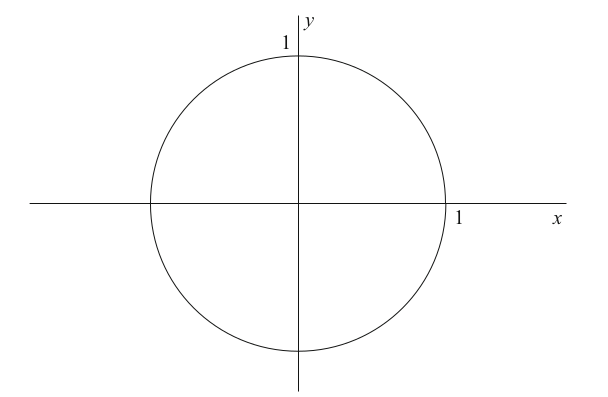
\includegraphics[width=0.50\textwidth]{circle.png}
    \caption{}
    \label{fig: }
  \end{center}
\end{figure}



\subsubsection{Example 2}
The variety $\mathrm{V((x^2+y^2-1)(3x+6y-4)) \subseteq R^2}$ defines all the points satisfying the circle of radius 1 centered at the origin and the line defined by the equation  (3x+6y-4):
\begin{figure}[H]
  \begin{center}
    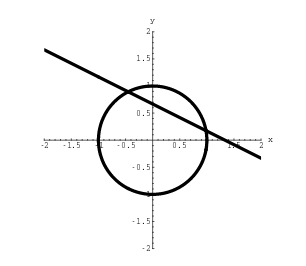
\includegraphics[width=0.50\textwidth]{circle_and_line.png}
    \caption{}
    \footnote{https://ocw.mit.edu/courses/electrical\-engineering\-and\-computer\-science/6\-972\-algebraic\-techniques\-and\-semidefinite\-optimization\-spring\-2006/lecture\-notes/lecture\_13.pdf}
    \label{fig: }
  \end{center}
\end{figure}


\subsection{Ideal}
Ideal is an algebraic object. The real importance of ideals is that they will give us a language for computing with affine varieties.In the next section we will define relation between polynomials, varieties (geometric object) and ideals (algebraic objects).\newline

\textbf{Definition 1 :}\newline
R is a commutative ring, a subset $\mathrm{ I \subseteq k[x_1,...,x_n] }$ ($\mathrm{ I \subseteq R }$) is an \textbf{Ideal} if it satisfies :
\begin{enumerate}
\item $\mathrm{0 \in I}$
\item $\mathrm{f,g \in I \implies f+g \in I}$
\item $\mathrm{f \in I, h \in G,\implies h.f \in I  }$
\end{enumerate}

\textbf{Example 1 :}\newline  (Z,+,.) is a commutative ring , Even numbers (2Z,+,.) is an ideal.\newline


\textbf{Definition 2 :}\newline
Let $\mathrm{ f_1,...,f_s }$ be a polynomial ring , in other words, be polynomials in  $\mathrm{ k[x_1,...,x_n] }$  then we set
\begin{equation}
  \langle f_1,..,f_s \rangle=\{ \sum_{i=1}^{s}{h_i.f_i}| h_1,...,h_s \in k[x_1,...,x_n]\}
\end{equation}
$\mathrm{ \langle f_1,..,f_s \rangle  }$ is an ideal \textbf{generated by} $\mathrm{f_1,..,f_s \in k[x_1,...,x_n]}$. \newline


\subsection{Relation Between Algebra and Geometry}

\textbf{Proposition 1 :}\newline
if $\mathrm{ f_1,...,f_s }$ and $\mathrm{ g_1,...,g_t }$ are bases of the same ideal in the ring $\mathrm{k[x_1,...,x_n] }$ so that $\mathrm{ \langle f_1,..,f_s \rangle = \langle g_1,..,g_t \rangle }$, then we have  $\mathrm{V(f_1,...,f_s)=V(g_1,...,g_t) }$ \newline

 \textbf{Example 1 :}\newline
As an example, consider the variety $\mathrm{V(2x^2+3y^2-11,x^2-y^2-3)}$. \newline It is easy to show that $\mathrm{\langle 2x^2+3y^2-11,x^2-y^2-3 \rangle = \langle x^2-4,y^2-1 \rangle }$  so that \newline $\mathrm{V(2x^2+3y^2-11,x^2-y^2-3)=V(x^2-4,y^2-1)=\{(+/-2,+/-1)\} }$ \newline
by the above proposition. Thus, by changing the basis of the ideal, we made it easier
to determine the variety.




\begin{figure}[H]
  \begin{center}
    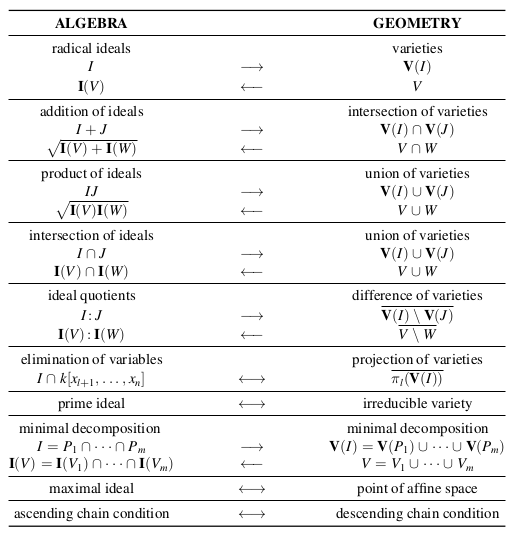
\includegraphics[width=0.95\textwidth]{algebra_geometry.png}
    \caption{}
    \label{fig: }
  \end{center}
\end{figure}

\section{Geometrical Meaning}

An affine variety $\mathrm{V(f_1 \ldots f_s)	\subset k^n}$ is the set of all solutions of the system of equations \\
 $\mathrm{f_1(x_1 \ldots x_n) = \ldots = f_s(x_1 \ldots x_n)}$ = 0. We will use the letters V,W,etc. to denote affine varieties. \cite{coxLittleOshea}
 \newline
 \newline
The conic sections studied in analytic geometry (circles, ellipses, parabolas) are affine varieties. Likewise, graphs of polynomial functions are affine varieties
[the graph of $\mathbf{y= f(x) \text{} \text{ is } \text{} V(y - f(x))}$].
Although not as obvious, graphs of rational functions are also affine varieties. For example, consider the graph of $\mathbf{y= \frac{x^3 -1}{x}}$ :

\begin{figure}[H]
  \begin{center}
    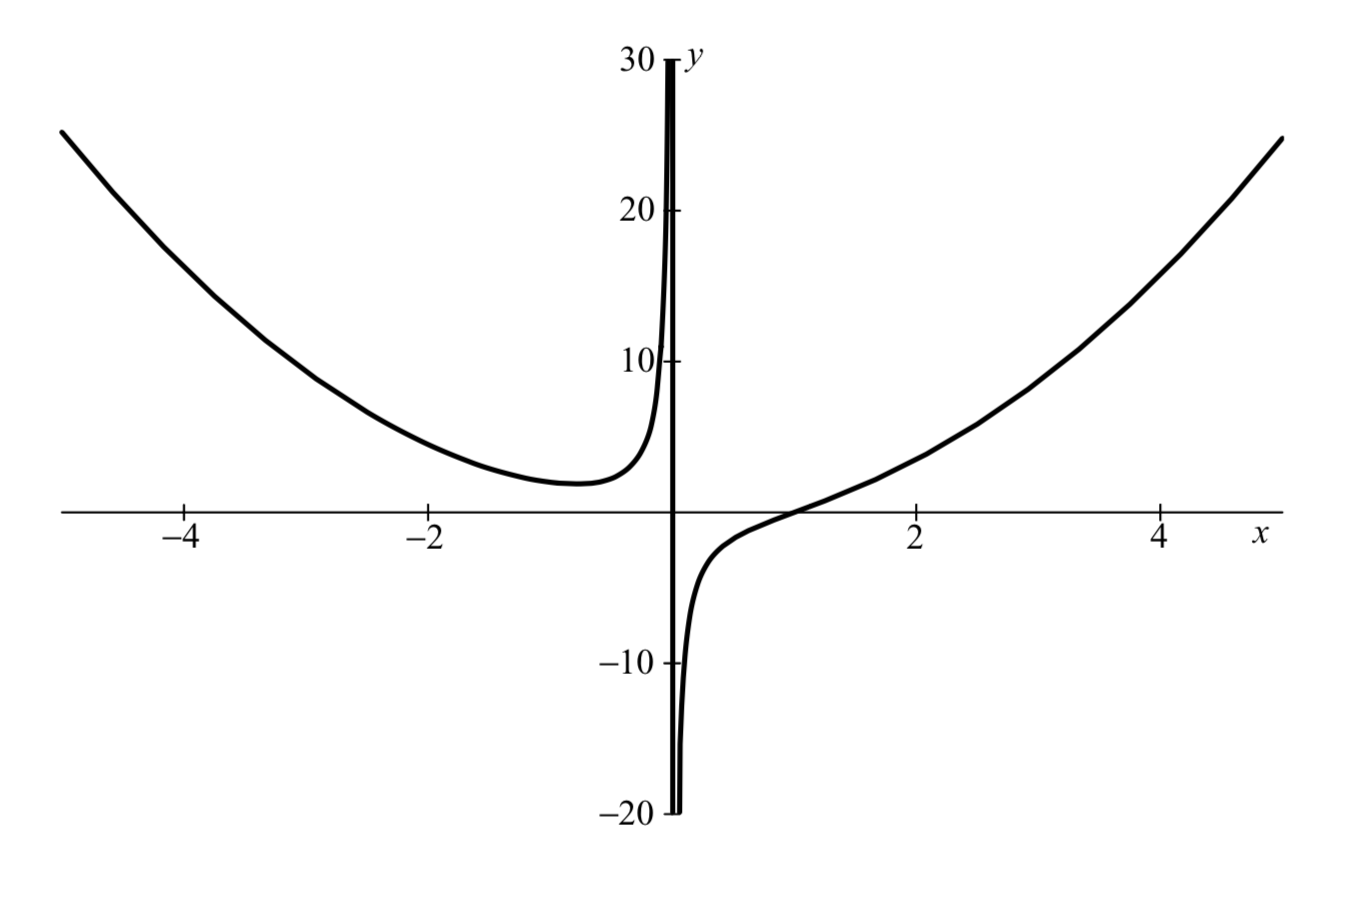
\includegraphics[width=0.50\textwidth]{conic.png}
    \caption{}
    \label{fig: }
  \end{center}
\end{figure}

3-dimensional space example. A nice affine variety is given by
paraboloid of revolution $\mathbf{V(z - x^2 - y)}$, which is obtained by rotating the parabola $\mathbf{z= x^2}$ about the z-axis.
This gives us the picture:

\begin{figure}[H]
  \begin{center}
    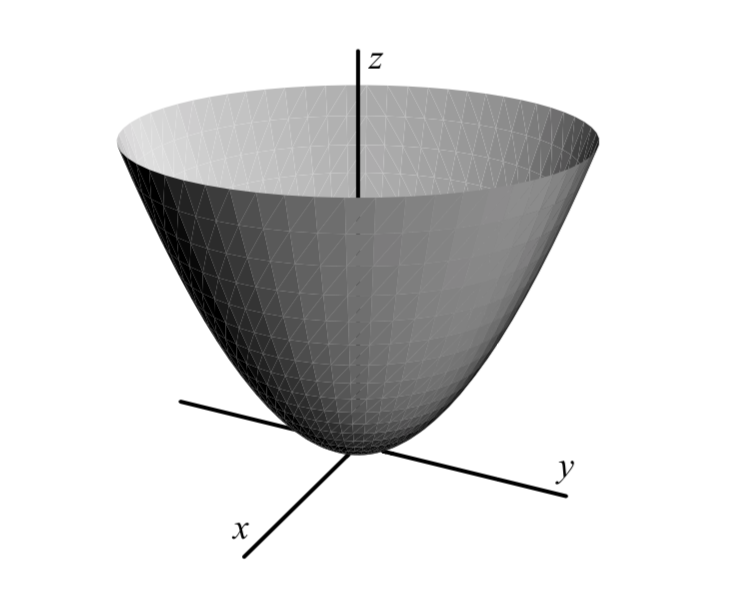
\includegraphics[width=0.50\textwidth]{threedimensinoal.png}
    \caption{}
    \label{fig: }
  \end{center}
\end{figure}

A much more complicated surface is given by $\mathbf{V(x^2 - y^2z^2 + z^3)}$:

\begin{figure}[H]
  \begin{center}
    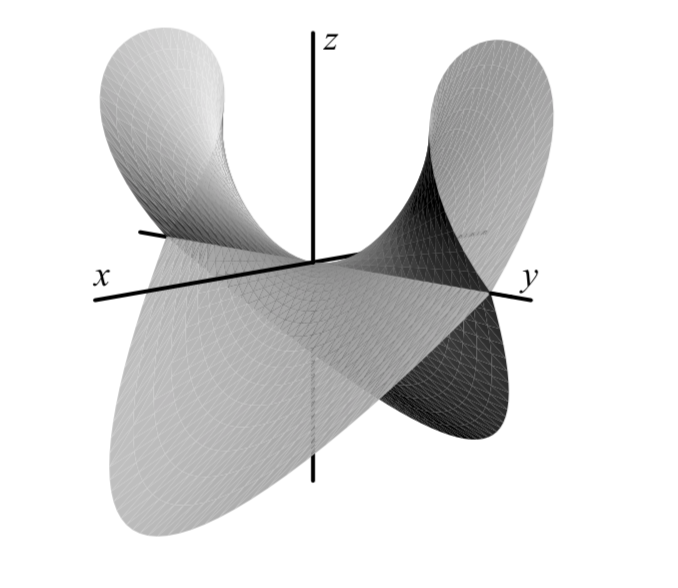
\includegraphics[width=0.50\textwidth]{complicated.png}
    \caption{}
    \label{fig: }
  \end{center}
\end{figure}

\section{Polynomial Systems Solution Methods}


\section{Solver Software}
There are many kind of solving softwares available for polynomial systems. We can separate them to two groups as native libraries and services.
Native libraries
In this section three libraries will be explained.
\subsection{Libraries}
\paragraph{Michael Thomas Flanagan's Java Scientific Library}

Flanagan library has many kind of operational functions, graph plotting, regression, polynomial operations, data smoothing etc.
This library has many useful advantages but use for commercial purposes isn't permitted.

\paragraph{M4GB}\cite{m4gbarticle}
is an  efficient algorithm for computing Grobner-Bases. It's an extension of Buchberger’s algorithm. It stores already computed (tail-)reduced multiplies of basis polynomials to prevent redundant work in reduction step. And it exploits efficient linear algebra for the reduction step.
They run a benchmark test with four libraries, OpenF4, FGb, Magma and M4GB. Others are different libraries to compute Grobner-Bases.
\begin{figure}[H]
  \begin{center}
    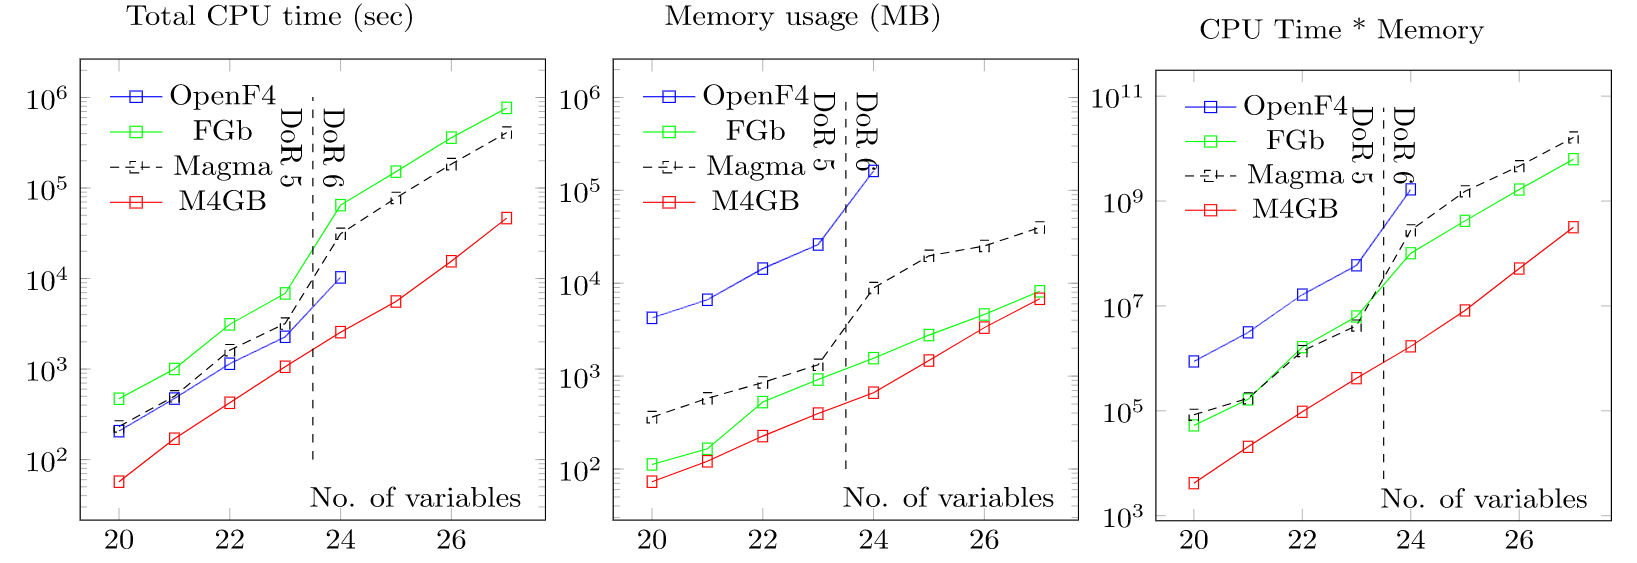
\includegraphics[width=\linewidth]{m4gb_m_2n.png}
    \caption{results for equations = variables * 2}
    \label{fig:m4gb_m_2n}
  \end{center}
\end{figure}

\begin{figure}[H]
  \begin{center}
    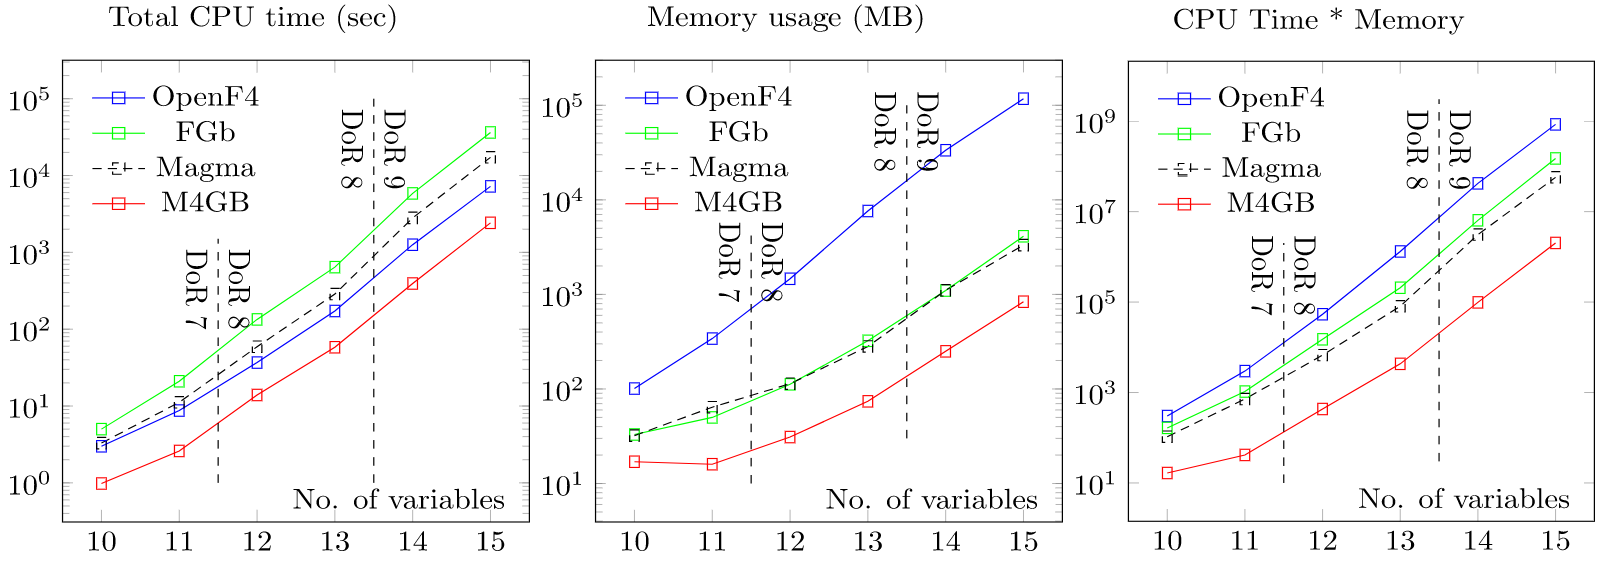
\includegraphics[width=\linewidth]{m4gb_m_n_1.png}
    \caption{results for equations = variables + 1}
    \label{fig:m4gb_m_n_1}
  \end{center}
\end{figure}
\section{Applications}
Systems of polynomial equations show up in many applications areas such as robotics (kinematics,motion planning, collision detection, etc.), computer vision (object modeling, surface fitting,recognition, etc.), graphics, geometric modeling (curve and surface intersections), computer-aided design, mechanical design, and chemical equilibrium systems. \cite{yanbinjiaArticle}
\subsection{Robotics}
System of polynomial equations may use to model a robot arm. If  ($\mathbf{x_i, y_i}$) is the coordinates of some joint,  ($\mathbf{x_i+1, y_i+1}$) is the coordinates of the next joint (or the hand) and the segment has length Li then we get the equation \cite{richterArticle}
\begin{figure}[H]
  \begin{center}
    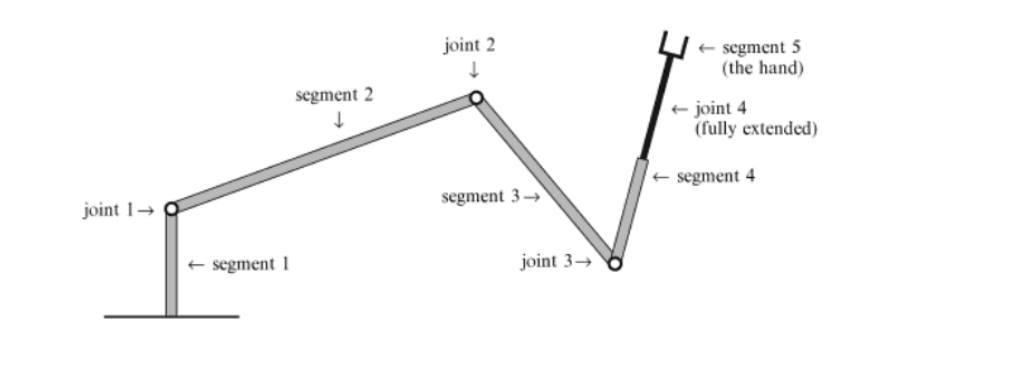
\includegraphics[width=0.70\textwidth]{robotarm.png}
    \caption{Robot Arm}
    \label{fig: Robot Arm}
  \end{center}
\end{figure}

 \begin{equation}
    (x_{i+1}-x_i)^2 + (y_{i+1}-y_i)^2=L_i^2
\end{equation}
Note that the angle at the i-th joint can be computed from the equations
 \begin{equation}
    x_{i+1}-x_i = L_i \cos(\theta_i)
\end{equation}
 \begin{equation}
    y_{i+1}-y_i = L_i \sin(\theta_i)
\end{equation}

\subsection{Geometry}
Many statements in Euclidean geometry can be formulated as result about systems of polynomial equations.\cite{richterArticle}

\textbf {Example:} Euclidean geometry says that \textit{the bisectors of the three sides of a triangle meet in one point.}

One vertex, A, of the triangle can be assumed to be the origin and another, B, to have coordinates (c, 0), without loss of generality. The third vertex, C, has coordinates (a,b).
The bisectors of AB and BC meet in some point, with coordinates (x1, y1). We get the following equations
\begin{equation}
    x_1- \frac {c}{2}=0
\end{equation}
\begin{equation}
    \frac {c-a}{b} \cdotp x_1 - y_1 + \frac {a^2 + b^2 - c^2}{2b} = 0
\end{equation}

Similarly, if (x2,y2) are the coordinates of the intersection of the bisectors of AB and AC we have
\begin{equation}
    x_2- \frac {c}{2}=0
\end{equation}
\begin{equation}
    \frac {a}{b} \cdotp x_2 + y_2 - \frac {b^2 + a^2}{2b} = 0
\end{equation}

\section{Conclusion}


\begin{thebibliography}{1}
\bibitem{berndStrumfelsBook}
  Strumfels Bernd,
  \textit{Solving Systems of Polynomial Equations},
   American Mathematical Society , Conference Board of Mathematical Sciences,
   Berkeley,CA,
   2002.
\bibitem{dineshManocaArticle}
  Manocha Dinesh,
  \textit{Solving Systems of Polynomial Equations},
   IEEE Computer Graphics and Applications
   University of North Carolina,
   1994.
\bibitem{hybridMethodArticle}
  L.H. Zhi and Y. Notake and H. Kai and M.-T. Noda and K.I. Shiraishi,
  \textit{Hybrid Method for Solving Polynomial Equations},
   Proceedings of the Asian Technology Conference in Mathematics, pp.492-501, Guangzhou, China, 1999.
\bibitem{gregoryBardThesis}
  Bard Gregory,
  \textit{Algorithms for Solving Linear and Polynomial Systems of Equations Over Finite Fields With Applications to Cryptanalysis},
   University of Maryland PHD Thesis,
   2007.
\bibitem{bettaleLukArticle}
  Luk Bettale 1 , Jean-Charles Faugère, Ludovic Perret,
  \textit{Solving multivariate polynomial systems over finite fields : Hybrid approach},
   Journées Nationales du Calcul Formel,
   UPMC, CNRS, INRIA Paris-Rocquencourt,
   2002.

\bibitem{morhacArticle}
   M. MORHAC,
  \textit{One-Modulus Residue Arithmetic Algorithm to Solve Linear Equations Exactly},
   Institute of Physics, Slovak Academy of Sciences
   Bratislava, Slovakia,
   1994.
\bibitem{emirisReport}
  I.Z. Emiris, A. Mantzaflaris, E. Tsigaridas,
  \textit{On the Bit Complexity of Solving Bilinear Polynomial Systems},
   Johan Radon Institute for Computational Mathematics,
   Austrian Academy Of Sciences,
   2016.
\bibitem{verscheldeArticle}
  Jan Verschelde,
  \textit{Homotopy Methods for Solving Polynomial Systems},
   ISSAC’05
   Beijing, China,
   2005.
\bibitem{courtoisaArticle}
  Nicolas Courtois , Alexander Klimov  , Jacques Patarin ,  Adi Shamir
  \textit{Efficient Algorithms for Solving Overdefined Systems of Multivariate Polynomial Equations},
   International Conference on the Theory and Applications of Cryptographic Techniques
   EUROCRYPT-2000,
   2000.
\bibitem{lazardArticle}
  Daniel Lazard,
  \textit{Thirty years of Polynomial System Solving, and now?},
   Journal of Symbolic Computation ,
   UPMC Univ. Paris, France,
   2008.
\bibitem{chenThesis}
  Changbo Chen,
  \textit{Solving Polynomial Systems via Triangular Decomposition},
   PHD Thesis
   The University of Western Ontario,
   2011.
\bibitem{faugereArticle}
  Jean-Charles Faugère, Pierrick Gaudry, Louise Huot, Guénaël Renault,
  \textit{Polynomial Systems Solving by Fast Linear Algebra},
   HAL <hal-00816724v1>,
   2013.
\bibitem{bondyfalatArticle}
  Didier Bondyfalat, Bernard Mourrain ,Victor Y. Pan
  \textit{Controlled iterative methods for solving polynomial systems},
   ISSAC 98 ,
   1998.
\bibitem{marinariArticle}
  M. G. MARINARI, H. M. MÖLLER, AND T. MORA
  \textit{ON MULTIPLICITIES IN POLYNOMIAL SYSTEM SOLVING},
   TRANSACTIONS OF THE AMERICAN MATHEMATICAL SOCIETY,
   1996.
\bibitem{chenArticle}
  Changbo Chen, Marc Moreno Maza,
  \textit{Algorithms for computing triangular decomposition of polynomial systems},
   Journal of Symbolic Computation,
   2012.
\bibitem{yienliArticle}
  Tien-Yien Li,
  \textit{SOLVING POLYNOMIAL SYSTEMS BY POLYHEDRAL HOMOTOPIES},
   TAIWANESE JOURNAL OF MATHEMATICS,
   1999.
\bibitem{duffArticle}
  Timothy Duff, Cvetelina Hill , Anders Jensen, Kisun Lee, Anton Leykin, Jeff Sommars,
  \textit{Solving polynomial systems via homotopy continuation and monodromy},
   CoRR,
   2017.
\bibitem{sommeseArticle}
  Andrew J. Sommese , Jan Verschelde , Charles W. Wampler ,
  \textit{Solving Polynomial Systems Equation by Equation},
   Dickenstein A., Schreyer FO., Sommese A.J. (eds) Algorithms in Algebraic Geometry,
   2006.
\bibitem{batesArticle}
  Dan Bates,
  \textit{Course Notes for Math 676: Computational Algebraic Geometry Spring 2009},
   Colorado State University,
   2009.
\bibitem{mouArticle}
  Chenqi Mou,
  \textit{Solving Polynomial Systems over Finite Fields:Algorithms, Implementation and Applications},
   HAL,
   Université Pierre et Marie Curie,
   2013.
\bibitem{alessioArticle}
  Caminata Alessio , Gorla Elisa.
  \textit{Solving Multivariate Polynomial Systems and an Invariant from Commutative Algebra. },
   2017.
\bibitem{abstractAlgebraBook}
  Karl-Heinz Fieseler,
  \textit{Groups, Rings and Fields },
   Upsalla
   2010.
\bibitem{richterArticle}
  Johan Richter,
  \textit{Systems of polynomial equations},
   2013.
\bibitem{wikipediaSystemofPolynomialEquations}
  \textit{ https://en.wikipedia.org/wiki/System\_of\_polynomial\_equations},
   Wikipedia,2018.

\bibitem{wolframPolynomial}
  \textit{ http://mathworld.wolfram.com/Polynomial.html},
   Wolfram,2018.
 \bibitem{yanbinjiaArticle}
  \textit{ https://pdfs.semanticscholar.org/295c/9b5d5e1120fdb3d5cf2386d8f6a92884d9f5.pdf},
   Yan-Bin Jia,2017.
\bibitem{m4gbarticle}
  Rusydi Makarim, Marc Stevens
  \textit{ M4GB: An Efficient Gröbner-Basis Algorithm},
   ISSAC 2017.
\bibitem{coxLittleOshea}
   Cox, Little, O'Shea,
   \textit{Ideals, Varieties, and Algorithms Book},
\end{thebibliography}


\end{document}
